\documentclass[a4paper]{article}
\usepackage{ucs}
\usepackage[utf8x]{inputenc}
\usepackage[T1]{fontenc}
\usepackage{german}
\usepackage{a4,ngerman}
\usepackage[ngerman]{babel}
\usepackage{graphicx}
\usepackage[]{cite}
\usepackage{fancyhdr}
\pagestyle{fancy}
\selectlanguage{german}
\usepackage{array}
\usepackage{mathtools}
\cfoot{\textcopyright Lukas Schörghuber, S1610307103}

\begin{document}
	\section{Kontrollfragen}
	
	\begin{enumerate}
		\item
		Eine Funktion gibt einen \textbf{eindeutigen} Zusammenhang zwischen ihren Termen an, z.B. stehen 2 und 3 im Addieren-Zusammenhang \textbf{nur} zu 5 und nicht zu 6.
		\newline
		Ein Prädikat gibt einen allgemeinen Zusammenhang zwischen seinen Termen oder Eigenschaften über seine Terme an, z.B. steht zwei im Kleiner-Zusammenhang sowohl zu 3 als auch zu 42.
		
		\item
		\begin{enumerate}
			\item Objekte
			\begin{equation*}
				42 \text{ ... Objektkonstante}
			\end{equation*}
			\begin{equation*}
				x \text{ ... Variable}
			\end{equation*}
			\begin{equation*}
				1180 \text{ ... Objektkonstante}
			\end{equation*}
		
			\item Funktionen
			\begin{equation*}
				\underbrace{f(\underbrace{2}_{\text{OK}}, \underbrace{1180}_{\text{OK}}, \underbrace{l}_{\text{V}})}_{\text{FK3}}
			\end{equation*}
			\begin{equation*}
				\underbrace{h(\underbrace{f(\underbrace{2}_{\text{OK}}, \underbrace{1180}_{\text{OK}}, \underbrace{l}_{\text{V}})}_{\text{FK3}}), \underbrace{*(\underbrace{y}_{\text{V}}, \underbrace{z}_{\text{V}})}_{\text{FK2}}}_{\text{FK2}}
			\end{equation*}
			\begin{equation*}
				\underbrace{/(\underbrace{h(\underbrace{f(\underbrace{2}_{\text{OK}}, \underbrace{1180}_{\text{OK}}, \underbrace{l}_{\text{V}})}_{\text{FK3}}), \underbrace{*(\underbrace{y}_{\text{V}}, \underbrace{z}_{\text{V}})}_{\text{FK2}}}_{\text{FK2}}), \underbrace{+(\underbrace{g(\underbrace{-(\underbrace{x}_{\text{V}}, \underbrace{z}_{\text{V}})}_{\text{FK2}}, \underbrace{5}_{\text{OK}}, \underbrace{x}_{\text{V}}, \underbrace{1180}_{\text{OK}})}_{\text{FK4}}, \underbrace{x}_{\text{V}})}_{\text{FK2}}}_{\text{FK2}}
			\end{equation*}
			
			\item Prädikate
			\begin{equation*}
				\underbrace{\geq(\underbrace{x}_{\text{V}}, \underbrace{1180}_{\text{OK}})}_{\text{PK2}}
			\end{equation*}
			\begin{equation*}
				\underbrace{P(\underbrace{+(\underbrace{x}_{\text{V}}, \underbrace{42}_{\text{OK}})}_{\text{FK2}}, \underbrace{1180}_{\text{OK}}, \underbrace{f(\underbrace{x}_{\text{V}}, \underbrace{1180}_{\text{OK}}, \underbrace{42}_{\text{OK}})}_{\text{FK3}})}_{\text{PK3}}
			\end{equation*}
			\begin{equation*}
				\underbrace{\text{isPrime}(\underbrace{x}_{\text{V}})}_{\text{PK1}}
			\end{equation*}
		\end{enumerate}
		
		\item
		I don't know.
		
		\item
		Junktoren werden benötigt, da Prädikatskonstanten nur Terme als Parameter akzeptieren, während Junktoren Wahrheitswerte, also die Ergebnisse der Prädikatkonstanten, verknüpfen.
		
		\item
		Variablen sind standardmäßig frei in einer Formel und werden durch die Verwendung eines Quantors auf genau dessen Ebene im Syntaxbaum gebunden.
		
		\item
		Ein Quantor akzeptiert zwei Parameter: die Variable, die gebunden wird und darauf folgend die Aussage. Ein Junktor verknüpft Wahrheitswerte, während eine FK bzw. PK nur Terme als Eingabeparameter akzeptieren.
		
		\item
		Das Universum legt fest, welchen Wertebereich Variablen annehmen können, welche Objektkonstanten definiert sind sowie die Stelligkeit der definierten FKs und PKs.
	\end{enumerate}
	
	\section{Aufgaben}
	
	\begin{enumerate}
		\item
		\begin{enumerate}
			\item
			\begin{equation*}
				\underbrace{\underbrace{\underbrace{3}_{\text{OK}} \cdot (\underbrace{4}_{\text{OK}} + \underbrace{x}_{\text{V}})}_{\text{FK2}} < \underbrace{\underbrace{x}_{\text{OK}} + \underbrace{y}_{\text{OK}}}_{\text{FK2}}}_{\text{PK2}}
			\end{equation*}
			\newline
			\begin{center}
				gültige atomare Aussage
			\end{center}
			
			\item
			\begin{equation*}
				\underbrace{Q(\underbrace{3}_{\text{OK}}, \underbrace{P(\underbrace{2}_{\text{OK}})}_{\text{PK1}})}_{\text{PK2}}
			\end{equation*}
			\newline
			\begin{center}
				Keine gültige Aussage, da Q einen Wahrheitswert als Parameter erhält.
			\end{center}
			
			\item
			\begin{equation*}
				\underbrace{\underbrace{g(\underbrace{5}_{\text{OK}}, \underbrace{\underbrace{5}_{\text{OK}} + \underbrace{3}_{\text{OK}}}_{\text{FK2}})}_{\text{FK2}} < \underbrace{\underbrace{x}_{\text{V}} + \underbrace{3}_{\text{OK}}}_{\text{FK2}}}_{\text{PK2}}
			\end{equation*}
			\begin{center}
				gültige atomare Aussage
			\end{center}
			
			\item
			\begin{equation*}
				\underbrace{\underbrace{P(\underbrace{x}_{\text{V}})}_{\text{PK1}} + \underbrace{Q(\underbrace{2}_{\text{OK}}, \underbrace{y}_{\text{V}})}_{\text{PK2}}}_{\text{FK2}}
			\end{equation*}
			\begin{center}
				Keine gültige atomare Aussage, da die FK + zwei Wahrheitswerte als Eingabeparameter erhält.
			\end{center}
			
			\item
			\begin{equation*}
				\underbrace{R(\underbrace{2}_{\text{OK}}, \underbrace{\underbrace{3}_{\text{OK}} + \underbrace{x}_{\text{V}}}_{\text{FK2}}, \underbrace{\underbrace{5}_{\text{OK}} \cdot \underbrace{y}_{\text{V}}}_{\text{FK2}})}_{\text{PK3}}
			\end{equation*}
			\begin{center}
				gültige atomare Aussage
			\end{center}
		\end{enumerate}
		
		\item
		\begin{enumerate}
			\item
			\begin{equation*}
				\underbrace{\underbrace{P(\underbrace{y}_{\text{V}})}_{\text{PK1}} < \underbrace{\underbrace{3}_{\text{OK}} + \underbrace{x}_{\text{V}}}_{\text{FK2}}}_{\text{PK2}}
			\end{equation*}
			\begin{center}
				Ungültige Aussage, da die PK > einen Term und einen Wahrheitswert als Eingabeparameter erhält.
			\end{center}
			
			\item
			\begin{equation*}
				\underbrace{\underbrace{f(\underbrace{x}_{\text{V}}, \underbrace{3}_{\text{OK}})}_{\text{FK2}} + \underbrace{g(\underbrace{f(\underbrace{x}_{\text{V}}, \underbrace{2}_{\text{OK}})}_{\text{FK2}}, \underbrace{4}_{\text{OK}})}_{\text{FK2}}}_{\text{FK2}}
			\end{equation*}
			\begin{center}
				Resultat ist ein gültiger Term.
			\end{center}
						
			\item
			\begin{equation*}
				\underbrace{\underbrace{f(\underbrace{\underbrace{3}_{\text{OK}} < \underbrace{4}_{\text{4}}}_{\text{PK2}}, \underbrace{y}_{\text{V}})}_{\text{FK2}} \cdot \underbrace{x}_{\text{V}}}_{\text{FK2}}
			\end{equation*}
			\newline
			\begin{center}
				Kein gültiger Term, da die FK f einen Wahrheitswert als Eingabeparameter erhält und daher ein ungültiges Ergebnis liefert.
			\end{center}
			
			\item
			\begin{equation*}
				\underbrace{Q(\underbrace{f(\underbrace{x}_{\text{V}}, \underbrace{3}_{\text{OK}}), \underbrace{  \underbrace{g(\underbrace{y}_{\text{V}})}_{\text{FK2}}+ \underbrace{2}_{\text{OK}}}_{\text{FK2}}}_{\text{FK2}})}_{\text{PK2}}
			\end{equation*}
			\begin{center}
				Ungültige Aussage, da die zweistellige Funktionskonstante nur einen Parameter erhält.
			\end{center}
			
			\item
			\begin{equation*}
				\underbrace{\underbrace{f(\underbrace{\underbrace{x}_{\text{V}} \cdot \underbrace{y}_{\text{V}}}_{\text{FK2}}, \underbrace{\underbrace{2}_{\text{OK}} \cdot \underbrace{y}_{\text{V}}}_{\text{FK2}})}_{\text{FK2}} < \underbrace{Q(\underbrace{2}_{\text{OK}}, \underbrace{y}_{\text{V}})}_{\text{PK2}}}_{\text{PK2}}
			\end{equation*}
			\begin{center}
				Ungültige Aussage, da die PK < einen Term und einen Wahrheitswert als Eingabeparameter erhält.
			\end{center}
		\end{enumerate}
		\clearpage
		
		\item
		\begin{enumerate}
			\item keine Quantoren vorhanden
			\begin{figure}[ht!]
				\begin{center}
					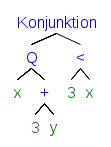
\includegraphics[height=45mm]{2a.png}
					\caption{Syntaxbaum für Aufgabe 3)a)}
				\end{center}
			\end{figure}
			
			\item keine Quantoren vorhanden
			\begin{figure}[ht!]
				\begin{center}
					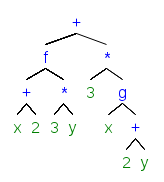
\includegraphics[height=45mm]{2b.png}
					\caption{Syntaxbaum für Aufgabe 3)b)}
				\end{center}
			\end{figure}
			
			\item Ask for assistance!
			\begin{figure}[ht!]
				\begin{center}
					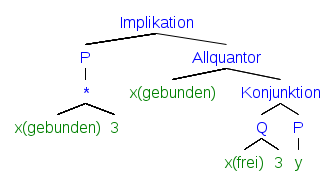
\includegraphics[height=45mm]{2c.png}
					\caption{Syntaxbaum für Aufgabe 3)c)}
				\end{center}
			\end{figure}
			\clearpage			
			
			\item ein Existenzquantor vorhanden
			\begin{figure}[ht!]
				\begin{center}
					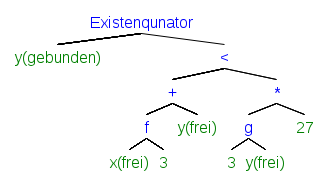
\includegraphics[height=45mm]{2d.png}
					\caption{Syntaxbaum für Aufgabe 3)d)}
				\end{center}
			\end{figure}
		\end{enumerate}
	\end{enumerate}
\end{document}